% !Mode:: "TeX:UTF-8"% !TEX TS-program = xelatex
% !TEX encoding = UTF-8 Unicode
% !Mode:: "TeX:UTF-8"

%+++++++++++++++++++++++++++++++++++++++++++++++++++++++++++++++++++++++++++++
% This is a sample article script. All rights reserved.
% Author: qianhui@zju.edu.cn
%+++++++++++++++++++++++++++++++++++++++++++++++++++++++++++++++++++++++++++++
\documentclass[a4paper,twoside,AutoFakeBold]{article}
% \usepackage{optreport}
\usepackage{./optreport}

%+++++++++++++++++++++++++++++++++++++++++++++++++++++++++++++++++++++++++++++
% Some packages for this sample.
%+++++++++++++++++++++++++++++++++++++++++++++++++++++++++++++++++++++++++++++
\usepackage{comment}	% Package for comment useless document
\usepackage{bm}			% Package for Bold-math symbol
\usepackage{mathrsfs}	% Package for RSFS fonts in maths
\usepackage{listings}	% Package for Listing code
\usepackage{enumerate}	% Package for enumerate
\usepackage{pdfrender}
\usepackage{subcaption}
\usepackage{multirow}
\usepackage{booktabs}
\usepackage{bbm}
\usepackage{bbding}
\usepackage{mathtools}
\usepackage{graphicx}
\usepackage{float}
\usepackage{epstopdf}
\usepackage{lipsum}
\usepackage{metalogo}

%+++++++++++++++++++++++++++++++++++++++++++++++++++++++++++++++++++++++++++++
% Title, Authors, Reprot Time.
%+++++++++++++++++++++++++++++++++++++++++++++++++++++++++++++++++++++++++++++
\serialnum{2020-3-109315041}

\rptname{Beck2009fast: A fast iterative shrinkage-thresholding algorithm for linear inverse problems}

\rptauthora{李淳风}{109315041} %作者1和学号
\rptauthorb{袁天罡}{109315042} %作者2和学号

\reporttime{2026}{1}

% -------------------------------------------------
% for english version.
% -------------------------------------------------
\rptcontentsname{Contents}
\renewcommand{\abstractname}{{\xiaosan Abstract}}
\def\bibetal{et al.}
\def\biband{and}
\makeatletter
\renewcommand*{\ALG@name}{{\xiaosi Algorithm.~}}
\makeatother
\theoremstyle{definition}
\newtheorem{defn2}{{Definition}}
\newtheorem{corr2}{{Corrollary}}
\newtheorem{thrm2}{{Theorem}}
\newtheorem{lema2}{{Lemma}}
\newtheorem{exmp2}{{Example}}
\newtheorem{remark2}{{Remark}}
\renewcommand*{\proofname}{{\heiti Proof.~}}
\renewcommand{\figurename}{Fig.~}
\renewcommand{\tablename}{Tab.~}
\renewcommand{\refname}{Reference}
% -------------------------------------------------
%+++++++++++++++++++++++++++++++++++++++++++++++++++++++++++++++++++++++++++++
% Document.
%+++++++++++++++++++++++++++++++++++++++++++++++++++++++++++++++++++++++++++++
\begin{document}
\pagenumbering{gobble}
%-----------------------------------------------------------------------------
%  Title Page
%-----------------------------------------------------------------------------
\maketitle
\thispagestyle{empty} % \cleardoublepage
\newpage
%-----------------------------------------------------------------------------
%  Table of Content
%-----------------------------------------------------------------------------
\rptcontent \thispagestyle{empty} % \cleardoublepage
\newpage
%-----------------------------------------------------------------------------
%  Abstract
%-----------------------------------------------------------------------------
% \begin{abstract}\kaiti \xiaosi
% \lipsum[3]
% \end{abstract}
% \cleardoublepage
%-----------------------------------------------------------------------------
%  Sections
%-----------------------------------------------------------------------------
\pagenumbering{arabic}\songti\xiaosi
%-----------------------
%
%-----------------------
\section{论文研究的问题背景}
\lipsum[6]

A popular family of optimization algorithms are so-called gradient descent algorithms: iterative algorithms that are com- prised of a gradient descent step at each iteration, followed by a projection step when there is a feasibility constraint. The purpose of the projection is to ensure that the update vector remains within the feasible set \cite{nesterov2013introductory}.

\citeauthor{wu2016decentralized} proposed a new method which using a stochastic strategy to pro-fuction the belief.
\[
a = \sum_0^1 f(x,y).
\]


\subsection{Using MS Word}
\lipsum[0]

\subsection{About Rating}
\lipsum[2]
\begin{enumerate}[(1)]
\item \lipsum[5]
\item \lipsum[7]
\end{enumerate}

\lipsum[8]

\subsection{Oganization}
\lipsum[9]

{
\color{blue} %
\lipsum[10] %
}

%-----------------------
%
%-----------------------
本节主要描述处理的问题,并解释常用的记号。

{\color{blue} 例如,分布式优化问题是一类重要的计算问题,在机器学习领域有大量的应用。分布式优化问题可以描述为如下形式。
\begin{equation}\label{eq:formulation}
\min_{x \in Q} \sum_{j \in \mathcal{N}} f_j(x).
\end{equation}
在式(\ref{eq:formulation})中,$Q$是约束集合;$\mathcal{N}$是一个网络节点的索引集合;$f_j$是在$j$节点上的目标函数。
}

\lipsum[7]

%-----------------------
%
%-----------------------

\section{论文的贡献}\label{section:contributions}


\section{论文的章节组织}\label{section:structure}



\section{论文的相关工作}\label{section:relation}

在相关工作以及其他任何章节,我们可以引用文献来说明相关的工作。

{\color{blue}
例如,我们可以如下撰写。
在\citeyear{nesterov2013introductory}年,\citeauthor{nesterov2013introductory}撰写了关于凸优化基本原理的教材\cite{nesterov2013introductory}。此后,一种简单的有限和最小化问题的简单加速算法被提出\cite{defazio2016simple},成为多种算法的基础\cite{eisen2017decentralized,davis2015convergence,colin2016gossip}。
%
由于算力的紧张,将优化计算分布在多个不同的计算节点上,成为优化领域的新方向。主要方法可以粗略地分为两条技术路线。第一条技术路线的代表性工作是DFISTA\cite{wu2016decentralized}...
}

\lipsum[6]

%-----------------------
%
%-----------------------

\section{论文的技术方法}\label{section:theory}


在本节中,算法可以表述如下算法~\ref{alg:thefirst}~所示。

\begin{algorithm}[h]\xiaosi
\caption{\xiaosi 计算 $y = x^n$}\label{alg:thefirst}
\begin{algorithmic} 
\REQUIRE $n \geq 0 \vee x \neq 0$
\ENSURE $y = x^n$
\STATE $y \leftarrow 1$
\IF{$n < 0$}
\STATE $X \leftarrow 1 / x$
\STATE $N \leftarrow -n$
\ELSE
\STATE $X \leftarrow x$
\STATE $N \leftarrow n$
\ENDIF
\WHILE{$N \neq 0$}
\IF{$N$ is even}
\STATE $X \leftarrow X \times X$
\STATE $N \leftarrow N / 2$
\ELSE[$N$ is odd]
\STATE $y \leftarrow y \times X$
\STATE $N \leftarrow N - 1$
\ENDIF
\ENDWHILE
\end{algorithmic}
\end{algorithm}

\lipsum[8]

\lipsum[9]

\lipsum[10]

%-----------------------
%
%-----------------------

\section{论文的实验结果}
请描述清楚实验的基本设置,例如:用何种数据集?参数是如何设定的?实验结果数据的来源(是自己做的实验还是引自他人的结果,如果是他人完成的实验,要注明参考文献)。建议要有实验的基本分析。实验的图的例子可参考图\ref{figure_LR_curves}。

\lipsum[25-26]
\begin{figure}[ht]
	\begin{subfigure}{.48\textwidth}
		\centering
		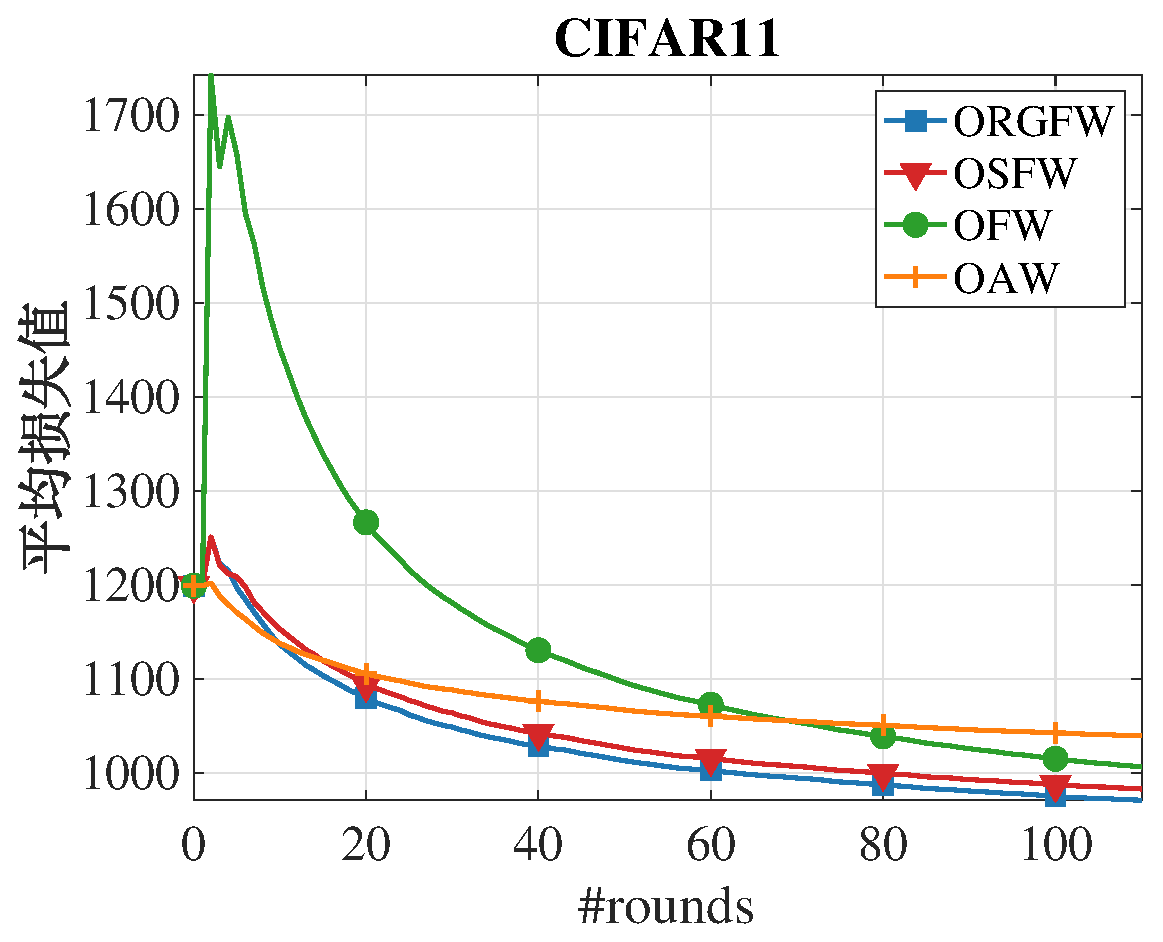
\includegraphics[width=\linewidth]{figs/CIFAR11_adv_regret}
	\end{subfigure}
	\hfill
	\begin{subfigure}{.48\textwidth}
		\centering
		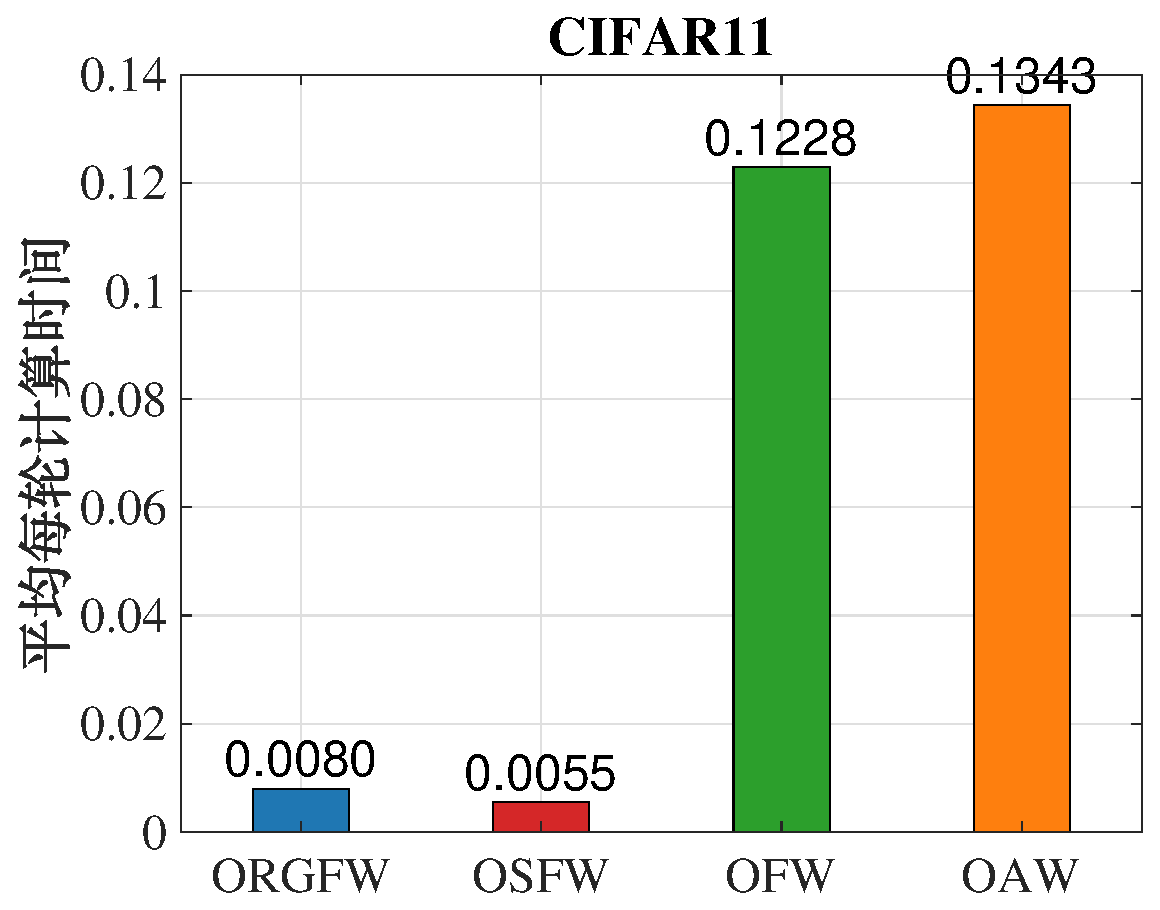
\includegraphics[width=\linewidth]{figs/CIFAR11_adv_time}
	\end{subfigure}
	\caption[在线多分类Logistic回归任务的实验结果]{
		在线多分类Logistic回归任务的实验结果。
		左边曲线图的横轴表示轮数,纵轴表示平均的损失函数值。
		右边的柱状图展示了每个算法平均每轮的计算时间。
	}
	\label{figure_LR_curves}
\end{figure}
\lipsum[27]

%-----------------------
%
%-----------------------
\section{论文的结论}

\lipsum[16]
\begin{defn2}[规范数]\label{defn:theone}
如果$x \in (0,1)$,则称$x$为规范数。
\end{defn2}
\begin{lema2}\label{lema:theone}
如果$x \in [0,1]$,则存在单调函数$\mathcal{G}(x)$ 有$\mathcal{G}(x) \geq f(x)$。
\end{lema2}
根据引理\ref{lema:theone}可以得到我们给出如下定理。
\begin{thrm2}\label{thrm:theone}
如果$x \in [0,1]$,则有$f(x) \geq f(y) + (x-y)^{\top} \nabla \mathcal{G}(x)$ 当且仅当 $f(\cdot)$是凸函数。
\end{thrm2}
根据定理\ref{thrm:theone}可以得到如下推论。
\begin{corr2}\label{corr:theone}
如果$x \in [0,1]$,则有$f(x)$是单调函数。
\end{corr2}
\begin{proof}
引理证明如下。
\end{proof}
\begin{exmp2}\label{corr:theone}
$f(x)= ax + b$,其中$a>0$。
\end{exmp2}

\begin{remark2}\label{remark:theone}
$f(x)$是单调函数。
\end{remark2}

\lipsum[28-29]
\subsection{收敛率相关理论结果}
\lipsum[31]
\subsubsection{光滑函数}
\lipsum[32]
\subsubsection{非光滑函数}
\lipsum[33]

\subsection{其他重要理论结果}
\lipsum[36]
\subsubsection{光滑函数}
\lipsum[34]
\subsubsection{非光滑函数}
\lipsum[35]

%-----------------------
%
%-----------------------
\section{论文存在的问题}\label{section:problem}




\section{围绕这篇论文可以开展哪些可行的研究}\label{section:application}
阐述上述理论有哪些应用,可以列举使用了上述理论的论文、专利、软硬件产品等。

\lipsum[16-24]

%-----------------------
%
%-----------------------



\lipsum[28]


%+++++++++++++++++++++++++++++++++++++++++++++++++++++++++++++++++++++++++++++
% Bibliography
%+++++++++++++++++++++++++++++++++++++++++++++++++++++++++++++++++++++++++++++
\bibliographystyle{gbt7714-plain}
\bibliography{main}

%+++++++++++++++++++++++++++++++++++++++++++++++++++++++++++++++++++++++++++++
\end{document}
%+++++++++++++++++++++++++++++++++++++++++++++++++++++++++++++++++++++++++++++


